% ------------------------------------------------------------------------------
% TYPO3 v9 LTS - What's New (German Version)
%
% @license	Creative Commons BY-NC-SA 3.0
% @link		https://typo3.org/help/documentation/whats-new/
% @language	German
% ------------------------------------------------------------------------------

\section{Admin Panel}
\begin{frame}[fragile]
	\frametitle{Admin Panel}

	\begin{center}\huge{\color{typo3darkgrey}\textbf{Admin Panel}}\end{center}
	\begin{center}\large{\textit{An insight into the internal processes of TYPO3 at run-time}}\end{center}

\end{frame}

% ------------------------------------------------------------------------------
% Admin Panel

\begin{frame}[fragile]
	\frametitle{Admin Panel}
	\framesubtitle{Admin Panel Überholung}

    Das Admin Panel wurde einer Generalüberholung unterzogen, um auf dem neuesten 
    Stand zu sein.
	\newline\newline
	Das Admin Panel wird im Frontend am Ende einer TYPO3 Seite angezeigt. Die Umschalttaste 
	auf der rechten Seite ermöglicht Integratoren und Editoren das Aktivieren und Deaktivieren
	des Admin Panels. Der folgende Screenshot zeigt den \textit{aktiven} Zustand.
	\vspace{0.8cm}
	\begin{figure}
		
\includegraphics[width=0.90\linewidth]{AdminPanel/AdminPanelEnabled.png}
	\end{figure}

\end{frame}

% ------------------------------------------------------------------------------
% Admin Panel: TypoScript Options

\begin{frame}[fragile]
	\frametitle{Admin Panel}
	\framesubtitle{Admin Panel: TypoScript Optionen}

	Der folgende Screenshot zeigt TypoScript-Optionen.

	\begin{figure}
		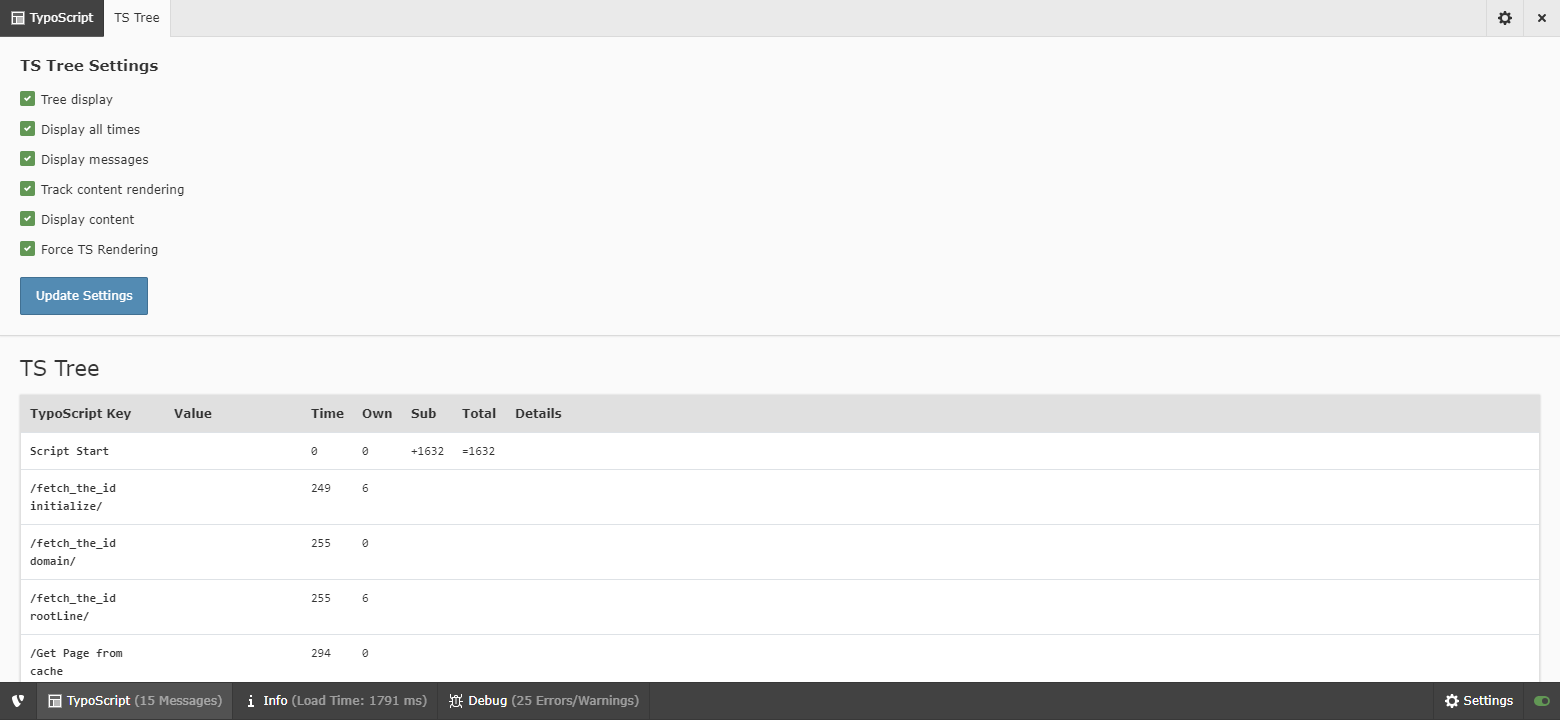
\includegraphics[width=0.90\linewidth]{AdminPanel/AdminPanelTypoScript.png}
	\end{figure}

\end{frame}

% ------------------------------------------------------------------------------
% Admin Panel: Configuration Options

\begin{frame}[fragile]
	\frametitle{Admin Panel}
	\framesubtitle{Admin Panel: Einstellungsmöglichkeiten}

	Der folgende Screenshot stellt Konfigurationsoptionen dar ("Settings").

	\begin{figure}
		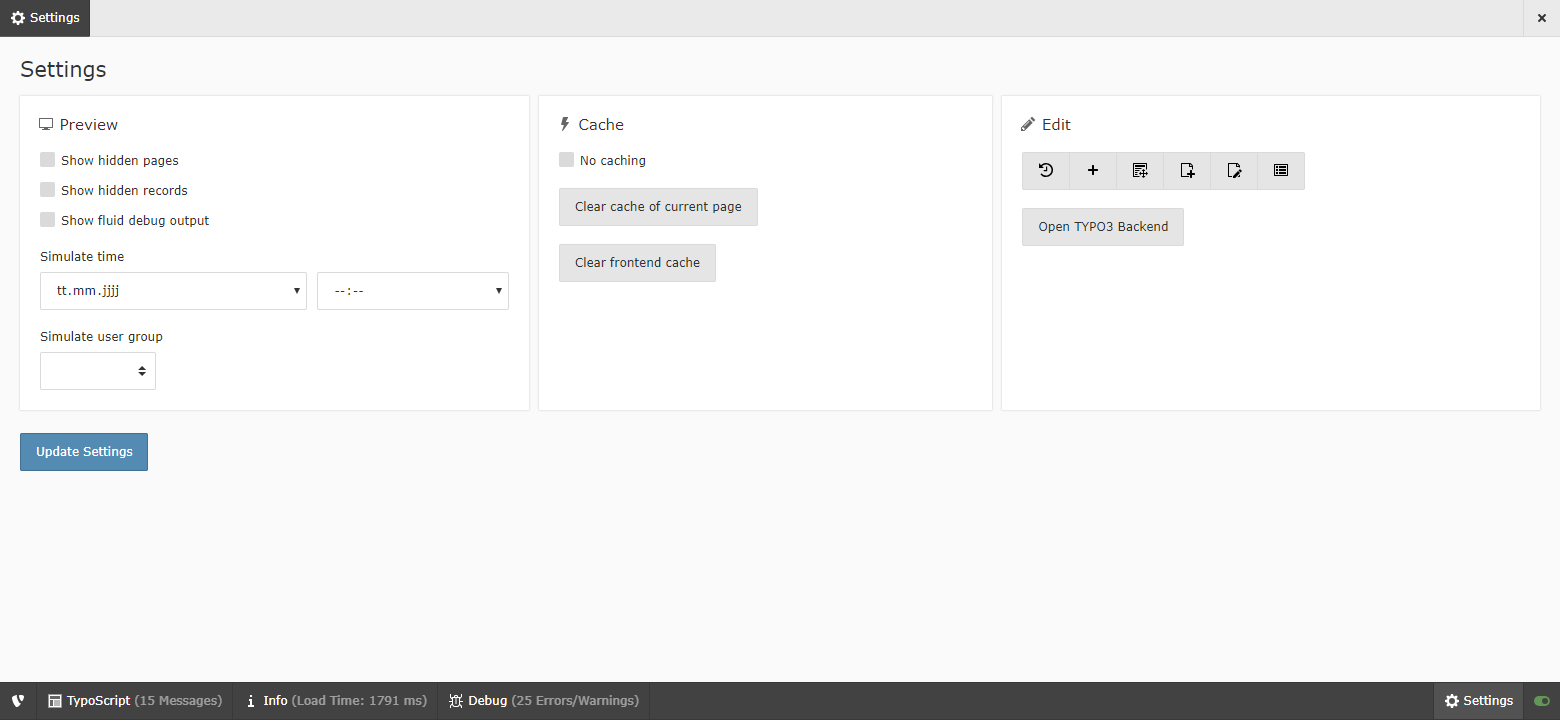
\includegraphics[width=0.90\linewidth]{AdminPanel/AdminPanelSettings.png}
	\end{figure}

\end{frame}

% ------------------------------------------------------------------------------
